\documentclass[preprint]{ltugproc}
\usepackage{mflogo,switcheml}
\usepackage[pdftex]{graphicx}

\bibliographystyle{ltugbib}

\title{Automatic Generation of Math Fonts for \TeX}

\author{Charles Duan}
\address{Harvard University \\ Cambridge, Massachusetts \\ USA}
\netaddress{\switchemail{cduan@eecs.harvard.edu}}

\divide\textheight\baselineskip \multiply\textheight\baselineskip

\begin{document}

\begin{abstract}
It is easy to use different fonts with \TeX, and writers of technical documents
enjoy this typographic flexibility. Unfortunately, there are few full math font
sets available, and the current practice of mixing incompatible text and math
fonts produces undesirable results. We describe a system that can automatically
produce a set of math fonts immediately suitable for typesetting with \TeX, such
that those math fonts are compatible with a given text font. This font generator
is designed to run automatically and without any technical knowledge on the part
of the end-user. Using this system, a wide variety of mock math fonts can be
generated, even for sans-serif fonts, and to great precision.
\end{abstract}

\maketitle

\section{Introduction}

Users of \TeX\ are fans of high-quality typesetting and fine typography, and
fans of fine typography enjoy the use of well-chosen, beautiful fonts for their
documents. Digital fonts are available in great quantity and high quality, but
these fonts nearly exclusively provide only the Roman alphabet. Of particular
interest to the current audience, there are only about five fonts complete with
mathematical symbols suitable for use with \TeX~\cite{bouche}. What is the poor
\TeX\-nician to do, given this abundance of text fonts and corresponding void of
mathematical symbols?

The most common option is to mix unrelated text and mathematics fonts. It is all
too common to see \emph{published} technical articles set in Times Roman text
but Computer Modern math. However, these unrelated fonts are often
\emph{visually incompatible}: dominant visual features of the two fonts are
inconsistent, and the reader is jarred and distracted by the visual
discontinuity. With regard to Times Roman and Computer Modern, the former has
thicker stems, less prominent serifs, and shorter capital letters than the
latter.

Naturally, the optimal solution would be for all of us to hire type designers to
make new, compatible math fonts for us on demand. Lacking the necessary
resources to do so, it seems that an \emph{automated approach to the creation of
compatible math fonts} is worth investigation.

\section{MathKit: A First Solution}

Alan Hoenig provided a first stab at a solution with
\emph{MathKit}~\cite{mathkit}. His system took advantage of one key observation:
the Computer Modern font programs, developed by Knuth~\cite{cte}, are
made up of sixty-two parameters that determine various visual elements of the
fonts they generate, so with the right set of parameters, a math font can be
\emph{automatically created} to match a given text font, and using virtual
fonts, the math symbols can be combined with the text font's italic letter set
to produce a highly compatible set of math fonts for use with \TeX\ or \LaTeX.

While MathKit is sufficient to generate compatible math fonts for many text
fonts, it has three main drawbacks. First, in order to create math fonts as
compatible with an arbitrary text font as possible, it is necessary to measure
many minute aspects of the text font. MathKit provides three parameter sets (for
Times Roman, Palatino, and Baskerville), but for other fonts the user must
create the parameter set alone---a task that, in the present author's
experience, involves learning the \MF\ language and carefully studying the
Computer Modern font programs in order to achieve good precision.

Second, even with a great deal of knowledge, several of the font parameters used
in the Computer Modern programs are difficult to measure by hand. For example,
several parameters define the amount of curvature of round letters; those
parameters are hard for a person to measure but fairly easy for a computer to
measure. (Naturally, there are also plenty of parameters that are easier for a
human to measure than a computer.) MathKit deals with these values by not
measuring them at all, simply taking the values out of Computer Modern's
standard parameter sets.

Third, a quality math font also requires proper spacing the characters (e.g.,
how much extra blank space to put on the left and right of each character).
MathKit provides a mechanism for setting these spacing values, but it makes no
attempt to set them automatically. Without proper spacing values, the letters
will rarely, if ever, be spaced correctly. However, given more than fifty-two
letters to adjust, the process of spacing adjustment is tedious, time-consuming,
and in general an unpleasant exercise.

\section{Motivation for a New System}

What we would like is a system for which a user without any formal knowledge of
typography or programming in general, let alone the specific implementations of
\MF\ and the Computer Modern programs, can produce math fonts reasonably
compatible with a given text font. The user should merely have to provide the
necessary font files, execute a program or two, and have a ready-to-use
collection of math symbols that match well with the text.

Naturally, an automatic system for generating aesthetically pleasing shapes can
do no better than an expert human designer, and it may not even surpass a
reasonably knowledgable non-expert. However, the calculated values should at
least provide a ballpark estimate. The automatic output should be acceptable for
use, and the determined user's task should be one of fine-tuning, adding and
subtracting small increments to already reasonable values, rather than one of
guessing values until the output looks reasonable.

\section{Design and Implementation}

The process of automatic math font generation requires two steps: measurement
and generation. In the measurement phase, the existing text font is analyzed,
producing a set of numerical (or other) parameters that will be fed to the
generation phase. In the generation phase, the set of parameters is applied to
font generation programs (in this case, a modified version of the Computer
Modern font programs) to create new math fonts.

\iffalse
In order to make this system extensible, the set of parameters passed between
the two stages must be as flexible as possible. In particular, it should be
relatively easy to add new parameters, as a greater number of parameters will
allow the font production to be more flexible and, hopefully, the resulting
fonts to be more compatible.
\fi

\subsection{The Measurement Phase}

We perform measurements on fonts in the Adobe Type~1 format. There are two good
reasons for this: first, Type~1 fonts are well-supported within
\TeX~\cite{lehman}; second, they are natively understood in the PostScript
language, so it is easy to perform analyses on them~\cite{plrm}.

The measurement routines are divided into two levels. First, a library of
``measurement primitives'' is given, providing simple functions such as finding
the intersection of a character's outline with a straight line or finding the
highest point in a character. Second, a set of measurement routines is built out
of that library, using those primitive actions to calculate the desired
parameter. For example, to measure the upright stem width of uppercase letters,
the program will draw a horizontal line 50\% through the height of the letter I,
find the (hopefully two) intersections between the line and the character
outline, and finally find the distance between those intersection points. For
each of (most of) the sixty-two parameters, one or more routines is used to
measure that parameter value (and multiple measurements are averaged according
to complex rules). Some parameters are also calculated based on several
measurements.

A thought that occurred to the author after he was more experienced in \MF\ (and
had already written the measurement routines) was that many of the primitives he
had written were built-in functions in \MF\ already. Thus, another way of
performing the measurements would be to translate the fonts into \MF\ (there are
programs to do this) and then perform measurements there. It may be worthwhile
translating the programs in this way if only for the speed increase (the
built-in \MF\ primitives would be much faster than the coded PostScript ones).

\subsection{The Generation Phase}

Once those parameters are calculated, they are passed to the font generation
programs. In most cases this is essentially like running MathKit with the
parameter set calculated from the measurement phase. However, there are two
differences.

First, many alterations have been made to the original Computer Modern font
programs. Many new parameters have been added to increase compatibility. Also,
several of the character designs, most notably $\beta$, $\gamma$, and $\delta$,
have been changed to permit for a wider parameter space. Additionally, Knuth
observes that the math symbol programs lack the ``metaness'' of the roman
letters; that is, much of their appearance is hard-coded rather than
determined by parameters. Several parameters have been introduced to provide
some more ``metaness.''

Second, the measurement phase also provides measurements for proper letter
spacing. The font generation process takes into account those spacing
measurements.

\section{Range of Font Support}

For which fonts can we automatically generate acceptable math fonts using this
procedure? In general, any font that looks relatively like Computer Modern will
produce a visually compatible math font. Additionally, support has been extended
to sans serif fonts. All of the standard Adobe printer fonts are supported:
Times Roman, Palatino, Bookman, New Century Schoolbook, Helvetica, Avant Garde,
and Courier. Many other fonts have been tested successfully; some samples will
be given below.

Fonts that will not work generally have one or more of the following qualities:
\begin{itemize}
\item They contain unexpected strokes or splotches of ink (e.g., a blackletter
font with two strokes for a capital I)
\item They have inconsistent stroke widths or character heights, or characters
that do not line up with the baseline (e.g., a very unusual handwriting font)
\item They tend to be used for display purposes instead of setting long passages
of text
\end{itemize}
Luckily, people tend not to want or need math fonts for unusual display
typefaces, so for any reasonable text font this program should be successful.

\section{Samples}

Below are several samples of generated math fonts. Please take the appearance
seriously, but not the content!

\begin{figure*}
\centering
\includegraphics[trim=112.1475pt 1.5in 112.1475pt 2in]{helvetica}
\end{figure*}

Helvetica demonstrates a number of features of the new fonts. First, notice the
new design of the $\delta$ character, whose top is flat rather than curved.
Also, the loops of the $\beta$ and other characters are squared off, as are many
of the terminals of letters. This ``squareness'' option is provided to the user;
fonts can be generated with either round or square ends.

\begin{figure*}
\centering
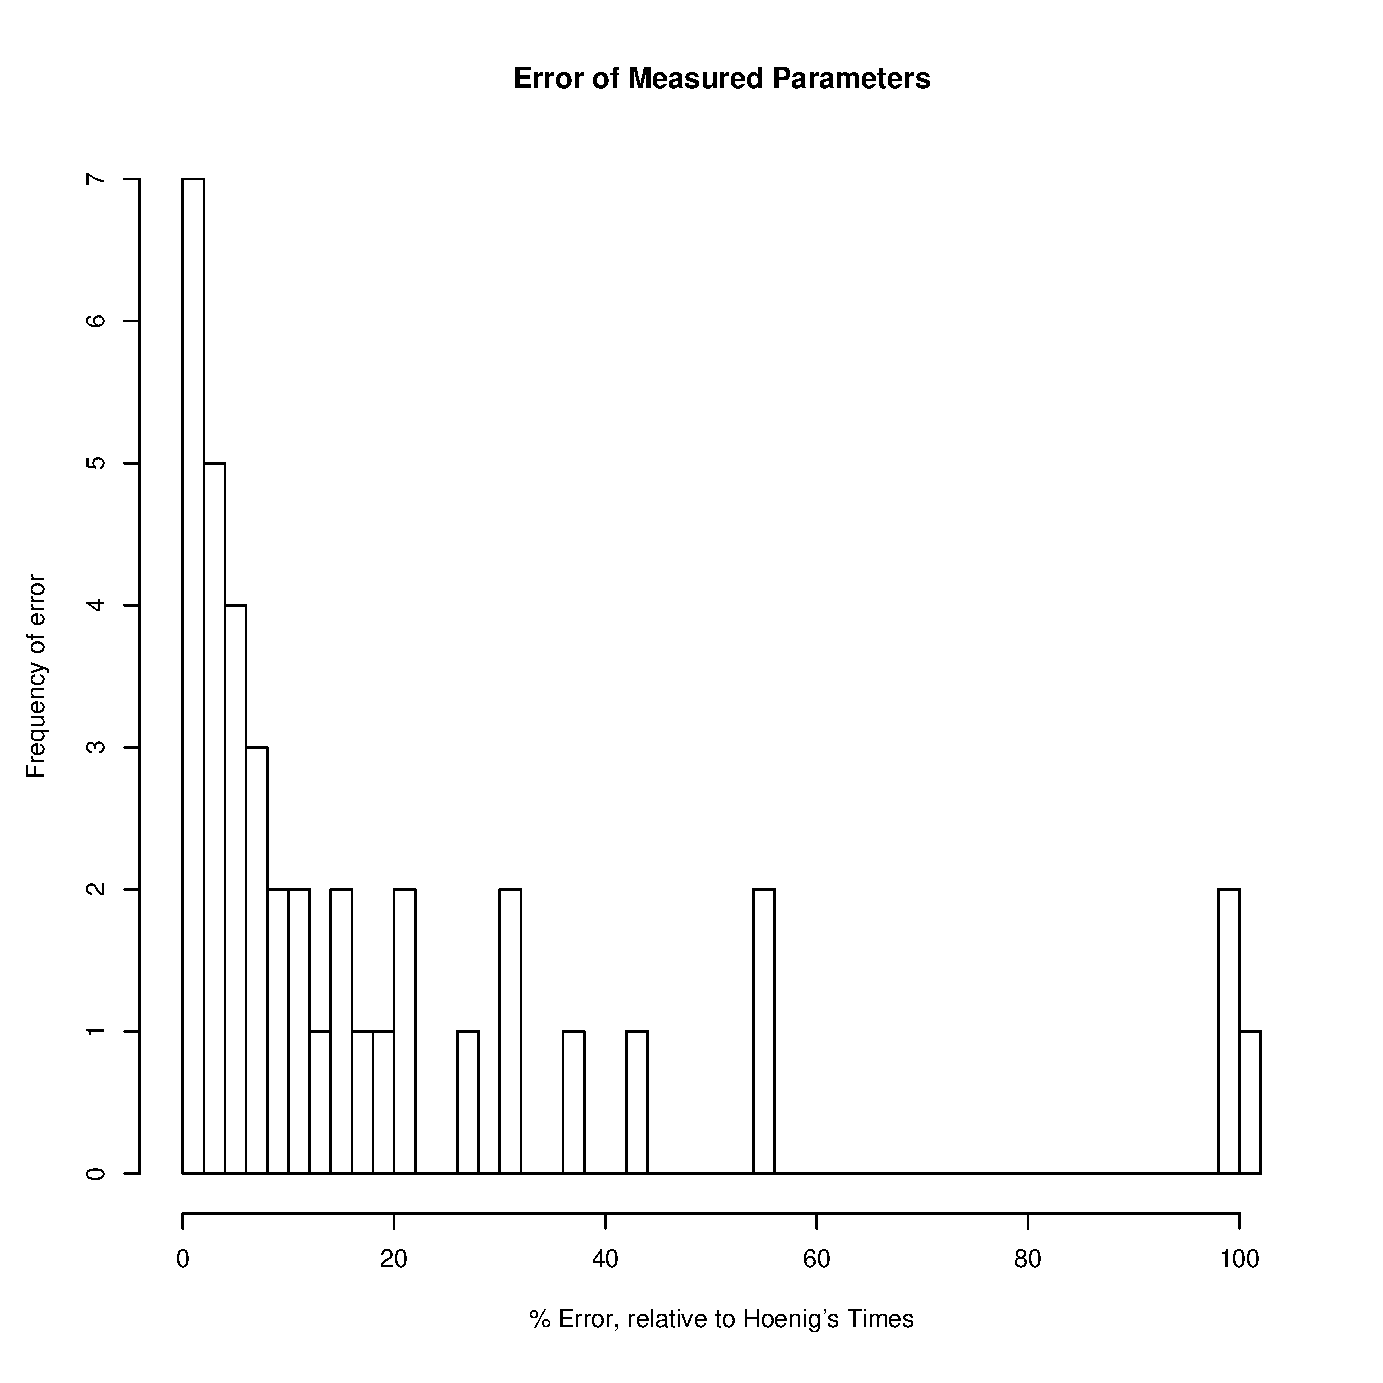
\includegraphics[trim=112.1475pt 1.5in 112.1475pt 2in]{times}
\end{figure*}

Times Roman displays a number of interesting features. The serifs are very thin
and short, as opposed to the relatively thick, prominent serifs of Computer
Modern. The generated $\Lambda$ and $\Gamma$ characters capture this, as do the
summation and product signs.

\begin{figure*}
\centering
%\fbox{\includegraphics[trim=112.1475pt 1.5in 112.1475pt 2in]{optima}}
\box0=\hbox{\lower 1.5in\vbox{\moveleft 112.1475pt \hbox{\includegraphics{optima}}}}
\ht0=8in \wd0=390pt
\leavevmode\box0
\end{figure*}

Optima is an interesting sans serif display font. The generated math characters
properly capture the stem width contrast and elegant flares. However, it is also
noteworthy what \emph{cannot} be captured: the minute flaring and slightly
curved terminals of the stems (compare the letters A and $\Lambda$). Qualities
that are not captured tend to be so small that they do not show up at small text
sizes, so for normal text (where mathematical symbols would most likely be used)
these minor insufficiencies are unnoticeable.

\section{Future Work}

In its current state, as exemplified by the samples above, high-quality math
symbol fonts can be produced for a wide variety of text fonts, and those symbols
typeset with quality comparable to hand-tuned characters. However, there are
several areas of potential and useful improvement.

First, the algorithms for performing spacing are somewhat na\"\i ve, measuring
only a sample of points and not taking into account any prior knowledge of the
shapes of characters. Better algorithms could be developed with some
investigation.

Second, the algorithm for calculating spacing could also be applied to
generating kerning pairs (fine adjustments to spacing between certain pairs of
characters).

Third, additional math fonts could be generated. MathKit provides blackboard
bold and Fraktur fonts; it should be possible to incorporate those as well.

Fourth, the math fonts are currently generated in bitmap form (as all \MF\
programs generate) and then traced using an outline tracing program to produce
Type~1 fonts. A better method would be to use \MP\ and various associated
utilities to produce Type~1 fonts without the tracing. This would require
rewriting the requisite \MF\ font generation programs a great deal, but in
theory the output fonts would be more efficient and appear better on digital
displays.

Finally, although the Computer Modern programs are sufficient for generating
very compatible math fonts, the resulting fonts tend not to have certain
distinctive features of the original text font. For instance, the small hooks or
serifs at the top and bottom of the stroke of the italic \emph{i} are very
distinctive for every font; such features should, optimally, be duplicated as
best as possible.

There are two good arguments \emph{against} duplicating such distinctive
features. First, those features are carefully crafted to the individual
letter, so a computer will not be able to successfully imitate them by some sort
of generic transformation. Second, the math symbols ought to look unique anyway,
so they might as well have different visual features.

Regardless of the camp in which you fall, there are two possible lines of work
stemming from this observation. First, new font generation programs need to be
written. Computer Modern was designed in a ``modern'' style; many of the
features of the modern type style (e.g. strong vertical stress; the lowercase
``o'' is symmetrical) are simply hard-coded into the font programs. It would be
interesting to develop a set of old-style font generation programs, for example,
one based on the Garamond fonts, but taking the same parameters for font design
variation. The end user could then choose whether to make a
Computer-Modern-style mock math font or a Garamond-style one; in both cases the
visual weight, character height, and other dominant aspects would match well,
but the style would differ.

Second, the current parameters are all numeric, with semantic meanings of
lengths, distances, or ratios of lengths or distances. What about a parameter
specifying a subpath of a character? For example, a ``parameter'' could be the
outline of the upper hook of the italic \emph{n}; that hook design could then be
adapted for generated characters such as $\eta$.

\section{Conclusion}

In an ideal world, every font designer would produce a full complement of math
fonts for every text font designed. In practice, the use of mathematical symbols
is sufficiently limited that math fonts are rarely designed. The automatic
generation of math symbol fonts by computerized measurements presents an ideal
alternative, producing high-quality math fonts without great difficulty.

Possibly the most interesting revelation of this work is the fact that
aesthetically pleasing math fonts can be produced by simple, static measurement
algorithms. In particular, it is not necessary to employ artificial intelligence
methods, even though the ultimate goal of the system is to produce output
comparable to what a human would produce. In a sense, this mirrors a major
contribution of \TeX\ itself: that aesthetics can, in many cases, be
discretized, quantified, and transformed into simple, deterministic algorithms.

\bibliography{fonts}

\end{document}
